\documentclass{templateNote}
\usepackage{soul}
\usepackage{fancyvrb}
\usepackage{fvextra}
\usepackage{enumitem}
\usepackage{xcolor,colortbl}

\definecolor{Verde}{RGB}{170,239,31}
\definecolor{Morado}{RGB}{127,0,255}
\definecolor{Celeste}{RGB}{0,191,255}
\definecolor{Salmon}{RGB}{255,0,157}

\begin{document}

\imagenlogoU{img/LogoElNube.png}
\linklogoU{https://github.com/MarceloPazPezo}
\linkQRDoc{https://github.com/MarceloPazPezo/MyRepo/blob/main/Icinf/Semestre\%207/Administraci\%C3\%B3n\%20y\%20Programaci\%C3\%B3n\%20de\%20Base\%20de\%20Datos/PL-SQL/PL-SQL\%20Oracle\%20XE.pdf}
\titulo{PL/SQL: Oracle Express Edition}
\asignatura{Administración y Programación de Base de Datos}
\autor{
    Marcelo Paz
}
\vDoc{1.1.0}

% Metadatos del PDF
\title{[\asignatura]-\titulo}
\author{
    \autor
}
\portada
\margenes % Crear márgenes

\section{Anotaciones}

\subsection{Crear otro usuario para la base de datos}

\begin{enumerate}
    \item Lo primero es permitir el uso de scripts en la sesión actual.
    \begin{figure}[H]
        \centering
        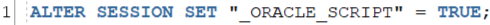
\includegraphics[width=0.5\textwidth]{img/image1.png}
    \end{figure}

    \item Luego en la conexión buscamos el directorio “Otros Usuarios”, le damos clic derecho y luego a “Crear Usuario…”.
    \begin{figure}[H]
        \centering
        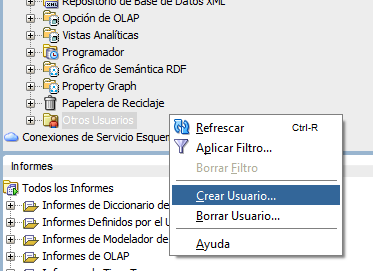
\includegraphics[width=0.5\textwidth]{img/image2.png}
    \end{figure}

    \item Le damos un nombre a nuestro nuevo usuario “USUARIOPRUEBA” y creamos una contraseña.
    \begin{figure}[H]
        \centering
        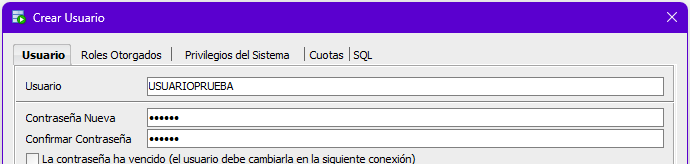
\includegraphics[width=0.8\textwidth]{img/image3.png}
    \end{figure}

    \newpage
    \item Nos vamos a la sección de “Roles Otorgados”, le damos a “CONNECT y DBA” y luego a “Aplicar”.
    \begin{figure}[H]
        \centering
        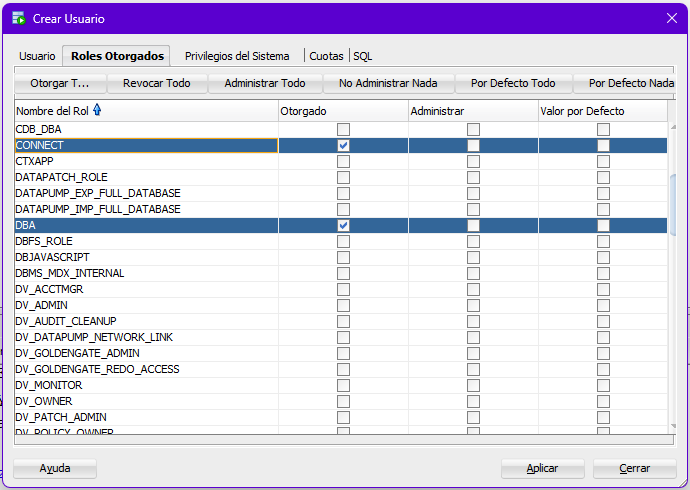
\includegraphics[width=0.7\textwidth]{img/image4.png}
    \end{figure}

    \item Debería aparecernos una ventana para confirmarnos el proceso.
    \begin{figure}[H]
        \centering
        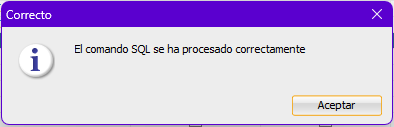
\includegraphics[width=0.5\textwidth]{img/image5.png}
    \end{figure}

    \item Para finalizar al crear una nueva conexión a la BD, debemos ingresar el usuario y darle a “Probar” para validar que la conexión se realiza correctamente (Borde Inferior Izquierdo nos muestra el “Estado: Correcto”).
    \begin{figure}[H]
        \centering
        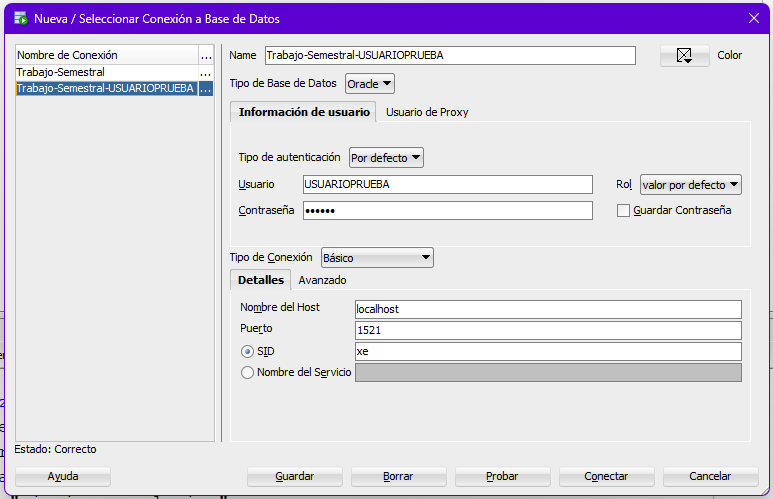
\includegraphics[width=0.7\textwidth]{img/image6.png}
    \end{figure}
\end{enumerate}

\subsection{[Extra] Tipos de la base de datos:}
\begin{itemize}
    \item Number(tamaño[,cantidadDecimales])
    \item CHAR(tamaño), VARCHAR2(tamaño)
    \item DATE
    \item LONG: bloque de texto (hasta 2GB)
    \item LONG RAW: Datos multimedia
    \item ROWID: Identificador único para cada fila.
\end{itemize}

\subsection{[Extra] Tipos de datos propios de PL/SQL:}
\begin{itemize}
    \item DEC, DECIMAL, REAL
    \item DOUBLE PRECISION, INTEGER
    \item BOOLEAN
    \item TABLE: similar a un arreglo
    \item RECORD: datos compuestos
    \item ...
\end{itemize}

\subsection{[Extra] Operadores}
\begin{itemize}
    \item Asignación: :=
    \item Aritméticos: +, -, *, /, MOD, ** (potencia)
    \item Relacionales: =, <>, >, <, >=, <=, ...
    \item Booleanos: AND, OR, NOT, ...
    \item Concatenación: ||
    \item ...
\end{itemize}

\subsection{[Extra] Palabras reservadas}
\begin{itemize}
    \item \textbf{BETWEEN:} Nos permite buscar valores entre dos valores.
    \item \textbf{ADD\_MONTHS(FECHA, N):} Nos permite sumar/restar 'N' meses a una FECHA.
    \item \textbf{COALESCE(COUNT(1), 0):} Nos permite contar los valores de una columna, si no hay valores, retorna 0.
    \item \textbf{EXTRACT(DAY/MONTH/YEAR FROM FECHA):} Nos permite extraer el d\'ia/mes/año de una FECHA.
\end{itemize}
\newpage
\section{PL/SQL}
\indent
De sus siglas en inglés \textbf{Procedural Language/Structured Query Language}, es un lenguaje de programación que añade funcionalidades a SQL, talez como programación por procedimientos.\\
\hl{Ventajas}:

\begin{itemize}
    \item Se administra centralmente dentro de la base de datos.
    
    \item Se comunica en forma nativa con objetos de la base de datos.
    
    \item Fácil de modularizar y manejar.
    
    \item Modularidad (Reusabilidad, esconder la complejidad)
    \begin{itemize}
        \item \textbf{Procedimientos:} Aceptan y retornan cero o más valores.
        \item \textbf{Funciones:} Aceptan y retornan un valor.
        \item \textbf{Triggers:} Sentencias asociadas a una tabla.
        \item \textbf{Paquetes:} Colección de procedimientos y funciones (definición y cuerpo).
    \end{itemize} 

\end{itemize}
\hl{Desventajas}:
\begin{itemize}
    \item Oracle.
\end{itemize}

\subsection{Estructura de un bloque PL/SQL}
Un bloque se compone de tres secciones:
\begin{enumerate}
    \item \textbf{Declaración de variables:} \begin{enumerate}
        \item Tipos Oracle
        \item Tipo exclusivo PL/SQL
    \end{enumerate}
    \begin{tcolorbox}[
        colframe=Celeste!100, % Color del borde
        colback=Celeste!20,       % Color del fondo
        coltitle=black!100, % Color del título
        title=\textbf{PL/SQL}, % Título de la caja
    ]
        \begin{verbatim}
DECLARE
    -- Declaración de variables
    nombre_variable tipo_dato;
    nombre_variable tipo_dato := valor;
        \end{verbatim}
    \end{tcolorbox}

    \newpage
    \item \textbf{Sección ejecutable:}
    \begin{itemize}
        \item Instrucciones a ejecutar dentro del bloque.
    \end{itemize}
    \begin{tcolorbox}[
        colframe=blue!100, % Color del borde
        colback=blue!20,       % Color del fondo
        coltitle=white!100, % Color del título
        title=\textbf{PL/SQL}, % Título de la caja
    ]
    \begin{Verbatim}[breaklines=true]
BEGIN
    -- Instrucciones
    nombre_variable := valor;
    nombre_variable := nombre_variable + 1;
        \end{Verbatim}
    \end{tcolorbox}


    \item (OPCIONAL) \textbf{Sección de manejo de excepciones:}
    \begin{itemize}
        \item Se definen los manejadores de errores que soportará el bloque.
    \end{itemize}
    \begin{tcolorbox}[
        colframe=Morado!100, % Color del borde
        colback=Morado!20,       % Color del fondo
        coltitle=white!100, % Color del título
        title=\textbf{PL/SQL}, % Título de la caja
    ]
    \begin{Verbatim}[breaklines=true]
EXCEPTION
    -- Manejo de excepciones
    WHEN nombre_excepcion THEN
        -- Instrucciones
        DBMS_OUTPUT.PUT_LINE('Error: ' || SQLERRM);
        \end{Verbatim}
    \end{tcolorbox}

    \item \textbf{Importante terminar con la palabra clave:}
    \begin{tcolorbox}[
        colframe=red!90!black, % Color del borde
        colback=red!20,       % Color del fondo
        coltitle=white!100, % Color del título
        title=\textbf{PL/SQL}, % Título de la caja
    ]
    \begin{Verbatim}[breaklines=true]
END;
        \end{Verbatim}
    \end{tcolorbox}
\end{enumerate}
El bloque completo se ve de la siguiente manera:
\begin{tcolorbox}[
    colframe=Verde!100, % Color del borde
    colback=Verde!20,       % Color del fondo
    coltitle=black!100, % Color del título
    title=\textbf{PL/SQL}, % Título de la caja
]
\begin{Verbatim}[breaklines=true]
DECLARE
    -- Declaración de variables
BEGIN
    -- Instrucciones
EXCEPTION
    -- Manejo de excepciones
END;
    \end{Verbatim}
\end{tcolorbox}

\newpage
\subsection{Estructuras de control}

\begin{itemize}
    \item \textbf{IF-THEN-ELSE:}
    \begin{tcolorbox}[
        colframe=Salmon!100, % Color del borde
        colback=Salmon!20,       % Color del fondo
        coltitle=black!100, % Color del título
        title=\textbf{PL/SQL}, % Título de la caja
    ]
        \begin{Verbatim}[breaklines=true]
IF (condicion) THEN
    -- Instrucciones
ELSIF (condicion) THEN
    -- Instrucciones
ELSE
    -- Instrucciones
END IF;
        \end{Verbatim}
    \end{tcolorbox}

    \item \textbf{GOTO:}
    \begin{tcolorbox}[
        colframe=Salmon!100, % Color del borde
        colback=Salmon!20,       % Color del fondo
        coltitle=black!100, % Color del título
        title=\textbf{PL/SQL}, % Título de la caja
    ]
    \begin{Verbatim}[breaklines=true]
GOTO <<etiqueta>>;
<<etiqueta>>:
    -- Instrucciones
        \end{Verbatim}
    \end{tcolorbox}

    \item \textbf{LOOP:}
    \begin{tcolorbox}[
        colframe=Salmon!100, % Color del borde
        colback=Salmon!20,       % Color del fondo
        coltitle=black!100, % Color del título
        title=\textbf{PL/SQL}, % Título de la caja
    ]
        \begin{Verbatim}[breaklines=true]
LOOP
    -- Instrucciones
    EXIT WHEN (condicion);
END LOOP;
        \end{Verbatim}
    \end{tcolorbox}

    \item \textbf{WHILE:}
    \begin{tcolorbox}[
        colframe=Salmon!100, % Color del borde
        colback=Salmon!20,       % Color del fondo
        coltitle=black!100, % Color del título
        title=\textbf{PL/SQL}, % Título de la caja
    ]
        \begin{Verbatim}[breaklines=true]
WHILE (condicion) LOOP
    -- Instrucciones
END LOOP;
        \end{Verbatim}
    \end{tcolorbox}

    \item \textbf{FOR:}
    \begin{tcolorbox}[
        colframe=Salmon!100, % Color del borde
        colback=Salmon!20,       % Color del fondo
        coltitle=black!100, % Color del título
        title=\textbf{PL/SQL}, % Título de la caja
    ]
        \begin{Verbatim}[breaklines=true]
FOR variable IN rango LOOP
    -- Instrucciones
END LOOP;
        \end{Verbatim}
    \end{tcolorbox}
\end{itemize}

\subsection{Procedimientos almacenados con varios argumentos}
Un procedimiento almacenado es un programa PL/SQL que tiene un nombre y ademas admite argumentos/parametros.

\begin{tcolorbox}[
    colframe=Morado!100, % Color del borde
    colback=Morado!20,       % Color del fondo
    coltitle=white!100, % Color del título
    title=\textbf{PL/SQL}, % Título de la caja
]
    \begin{Verbatim}[breaklines=true]
CREATE [OR REPLACE] PROCEDURE <PR_nom>(<pa1> [IN/OUT/IN OUT] <type>, <pa2> [IN/OUT/IN OUT] <type>,...)
RETURN tipo_dato
IS
    -- Declaración de variables locales
BEGIN
    -- Instrucciones
    RETURN valor;
[EXCEPTION]
    -- Manejo de excepciones
END;
    \end{Verbatim}
\end{tcolorbox}
OBS:
\begin{itemize}
    \item Las palabras en corchetes son opcionales.
    \item Las palabras en $< >$ son las variables/tipo de datos.
    \item Un parametro puede ser de entrada 'IN', salida 'OUT' o ambos 'IN OUT'.
\end{itemize}
\subsubsection{Ejecutar un procedimiento almacenado}
\begin{tcolorbox}[
    colframe=Morado!100, % Color del borde
    colback=Morado!20,       % Color del fondo
    coltitle=white!100, % Color del título
    title=\textbf{PL/SQL}, % Título de la caja
]
    \begin{Verbatim}[breaklines=true]
EXECUTE <PR_nom>(<valor1>, <valor2>, ...);
EXEC <PR_nom>(<valor1>, <valor2>, ...); -- Alternativa

BEGIN -- Alternativa
    <PR_nom>(<valor1>, <valor2>, ...);
END;
    \end{Verbatim}
\end{tcolorbox}

\subsubsection{Borrar un procedimiento almacenado}
\begin{tcolorbox}[
    colframe=red!90!black, % Color del borde
    colback=red!20,       % Color del fondo
    coltitle=white!100, % Color del título
    title=\textbf{PL/SQL}, % Título de la caja
]
    \begin{Verbatim}[breaklines=true]
DROP PROCEDURE <PR_nom>;
    \end{Verbatim}
\end{tcolorbox}

\newpage
\subsection{Manipulación de datos}
\begin{itemize}
    \item \textbf{INSERT:} para agregar datos.
    \begin{tcolorbox}[
        colframe=Verde!100, % Color del borde
        colback=Verde!20,       % Color del fondo
        coltitle=black!100, % Color del título
        title=\textbf{PL/SQL}, % Título de la caja
    ]
        \begin{Verbatim}[breaklines=true]
INSERT INTO nombre_tabla (columna1, columna2, ...)
VALUES (valor1, valor2, ...);
        \end{Verbatim}
    \end{tcolorbox}
*OBS: en Oracle no se puede multiples filas con un solo insert.
    
    \item \textbf{UPDATE:} para modificar datos.
    \begin{tcolorbox}[
        colframe=Verde!100, % Color del borde
        colback=Verde!20,       % Color del fondo
        coltitle=black!100, % Color del título
        title=\textbf{PL/SQL}, % Título de la caja
    ]
        \begin{Verbatim}[breaklines=true]
UPDATE nombre_tabla
SET columna1 = valor1, columna2 = valor2, ...
WHERE condicion;
        \end{Verbatim}
    \end{tcolorbox}

    \item \textbf{DELETE:} para eliminar datos.
    \begin{tcolorbox}[
        colframe=red!90!black, % Color del borde
        colback=red!20,        % Color del fondo
        coltitle=white!100, % Color del título
        title=\textbf{PL/SQL}, % Título de la caja
    ]
        \begin{Verbatim}[breaklines=true]
DELETE FROM nombre_tabla
WHERE condicion;
        \end{Verbatim}
    \end{tcolorbox}

    \item \textbf{DROP:} para eliminar tablas/trigger/procedimientos/indices/vistas.
    \begin{tcolorbox}[
        colframe=red!90!black, % Color del borde
        colback=red!20,       % Color del fondo
        coltitle=white!100, % Color del título
        title=\textbf{PL/SQL}, % Título de la caja
    ]
        \begin{Verbatim}[breaklines=true]
DROP TABLE nombre_tabla;
DROP TRIGGER nombre_trigger;
DROP PROCEDURE nombre_procedimiento;
DROP INDEX nombre_indice;
DROP VIEW nombre_vista;
        \end{Verbatim}
    \end{tcolorbox}
\end{itemize}

\newpage
\subsection{Cursores}
\indent
Controladores de áreas de memoria que almacenan los resultados de una instrucción SELECT.
\subsubsection{Tipos de cursores}
\begin{itemize}
    \item \textbf{Explícitos:} Se declara que es un cursor y luego se manipula para obtener 1 o varios valores.
    \begin{tcolorbox}[
        colframe=Salmon!100, % Color del borde
        colback=Salmon!20,       % Color del fondo
        coltitle=black!100, % Color del título
        title=\textbf{PL/SQL}, % Título de la caja
    ]
        \begin{Verbatim}[breaklines=true]
DECLARE
    CURSOR nombre_cursor IS
        SELECT columna1, columna2, ...
        FROM nombre_tabla
        WHERE condicion;
BEGIN
    OPEN nombre_cursor;
    FETCH nombre_cursor INTO variable1, variable2, ...;
    CLOSE nombre_cursor;
END;
        \end{Verbatim}
    \end{tcolorbox}
    \begin{itemize}[label={}]
        \item \begin{tcolorbox}[
            colframe=Celeste!100, % Color del borde
            colback=Celeste!20,       % Color del fondo
            coltitle=black!100, % Color del título
            title=\textbf{PL/SQL}: \textit{Abrir el cursor.}, % Título de la caja
        ]
            \begin{Verbatim}[breaklines=true]
    OPEN nombre_cursor;
            \end{Verbatim}
        \end{tcolorbox}
    \end{itemize}
    \begin{tcolorbox}[
        colframe=Celeste!100, % Color del borde
        colback=Celeste!20,       % Color del fondo
        coltitle=black!100, % Color del título
        title=\textbf{PL/SQL}: \textit{Recuperar los datos del Buffer.}, % Título de la caja
    ]
        \begin{Verbatim}[breaklines=true]
FETCH nombre_cursor INTO variable1, variable2, ...;
        \end{Verbatim}
    \end{tcolorbox}

    \begin{tcolorbox}[
        colframe=Celeste!100, % Color del borde
        colback=Celeste!20,       % Color del fondo
        coltitle=black!100, % Color del título
        title=\textbf{PL/SQL}: \textit{Cerrar el cursor.}, % Título de la caja
    ]
        \begin{Verbatim}[breaklines=true]
CLOSE nombre_cursor;
        \end{Verbatim}
    \end{tcolorbox}
    OBS:
    \begin{itemize}
        \item Un cursor explícito se debe abrir, recuperar y cerrar.
        \item Un cursor explícito admite par\'ametros (variables) para filtrar los datos.
        \item Si el cursor explícito recupera más de un valor, se debe usar un bucle.
    \end{itemize}

    \newpage
    \item \textbf{Implícitos:} Solo se declara la consulta y se recupera el un solo valor, por lo que si la consulta retorna más de un valor, se generará un error/excepci\'on.
    \begin{tcolorbox}[
        colframe=Salmon!100, % Color del borde
        colback=Salmon!20,       % Color del fondo
        coltitle=black!100, % Color del título
        title=\textbf{PL/SQL}: \textit{Cerrar el cursor.}, % Título de la caja
    ]
        \begin{verbatim}
DECLARE
    m amigos%ROWTYPE;
BEGIN
    SELECT * INTO m
    FROM amigos
    WHERE id = 1020;
    DBMS_OUTPUT.PUT_LINE('Mi amigo se llama'||m.nombre);
END;
        \end{verbatim}
    \end{tcolorbox}
    OBS:
    \begin{itemize}
        \item Un cursor implícito no se necesita abrir, recuperar o cerrar.
        \item En el ejemplo anterior, se recupera un solo valor pues suponemos que el ID es la clave primaria y por lo tanto hay un unico valor posible dentro de esta.
    \end{itemize}
\end{itemize}

\newpage
\subsubsection{Recorrer un cursor explícito}
\begin{tcolorbox}[
    colframe=Morado!100, % Color del borde
    colback=Morado!20,       % Color del fondo
    coltitle=white!100, % Color del título
    title=\textbf{PL/SQL}: \textit{Recorrer cursor con DO-WHILE.}, % Título de la caja
]
    \begin{verbatim}
DECLARE
    CURSOR misAmigos IS
        SELECT * FROM amigos;
    elAmigo amigos%ROWTYPE;
BEGIN
    OPEN misAmigos;
    LOOP
        FETCH misAmigos INTO elAmigo;
        EXIT WHEN misAmigos%NOTFOUND;
        DBMS_OUTPUT.PUT_LINE('Mi amigo se llama -->'||elAmigo.nombre);
    END LOOP;
END;
    \end{verbatim}
\end{tcolorbox}

\begin{tcolorbox}[
    colframe=Morado!100, % Color del borde
    colback=Morado!20,       % Color del fondo
    coltitle=white!100, % Color del título
    title=\textbf{PL/SQL}: \textit{Recorrer cursor con WHILE.}, % Título de la caja
]
    \begin{verbatim}
DECLARE
    CURSOR misAmigos IS
        SELECT * FROM amigos;
    elAmigo amigos%ROWTYPE;
BEGIN
    OPEN misAmigos;
    WHILE misAmigos%FOUND LOOP
        FETCH misAmigos INTO elAmigo;
        DBMS_OUTPUT.PUT_LINE('Mi amigo se llama -->'||elAmigo.nombre);
    END LOOP;
END;
    \end{verbatim}
\end{tcolorbox}

\begin{tcolorbox}[
    colframe=Verde!100, % Color del borde
    colback=Verde!20,       % Color del fondo
    coltitle=black!100, % Color del título
    title=\textbf{PL/SQL}: \textit{Recorrer cursor con FOR.}, % Título de la caja
]
    \begin{verbatim}
DECLARE
    CURSOR misAmigos IS
        SELECT * FROM amigos;
    elAmigo amigos%ROWTYPE;
BEGIN
    FOR elAmigo IN misAmigos LOOP
        DBMS_OUTPUT.PUT_LINE('Mi amigo se llama -->'||elAmigo.nombre);
    END LOOP;
END;
    \end{verbatim}
\end{tcolorbox}
*OBS: No se necesita abrir, recuperar o cerrar. Por lo que el utilizar un FOR es una forma implicita de recorrer el CURSOR.

\newpage
\subsubsection{Ejemplo}
Supongamos que tenemos la siguiente tabla:
\begin{center}
    \begin{tabular}{|c|c|c|c|}
        \hline
        \multicolumn{4}{|c|}{VEHICULO} \\ \hline
        ID & Marca & Tipo & Color \\
        \hline
        1 & Toyota & Auto & Rojo \\
        2 & Nissan & Auto & Verde \\
        3 & Mercedes & Camion & Blanco \\
        4 & Mercedes & Camion & Rojo \\
        \hline
    \end{tabular}
\end{center}
Programa 1: Mostrar los datos del veh\'icolo con ID = '3'.
\begin{tcolorbox}[
    colframe=Morado!100, % Color del borde
    colback=Morado!20,       % Color del fondo
    coltitle=white!100, % Color del título
    title=\textbf{PL/SQL}, % Título de la caja
]
    \begin{verbatim}
DECLARE
    vehiculoID VEHICULO.ID%ROWTYPE;
    vehiculoM VEHICULO.Marca%ROWTYPE;
    vehiculoT VEHICULO.Tipo%ROWTYPE;
    vehiculoC VEHICULO.Color%ROWTYPE;
BEGIN
    SELECT ID, Marca, Tipo, Color
    INTO vehiculoID, vehiculoM, vehiculoT, vehiculoC
    FROM VEHICULO
    WHERE ID = 3;
    DBMS_OUTPUT.PUT_LINE('Datos');
    DBMS_OUTPUT.PUT_LINE('      ID: ' || vehiculoID);
    DBMS_OUTPUT.PUT_LINE('    Marca: ' || vehiculoM);
    DBMS_OUTPUT.PUT_LINE('     Tipo: ' || vehiculoT);
    DBMS_OUTPUT.PUT_LINE('    Color: ' || vehiculoC);
END;
    \end{verbatim}
\end{tcolorbox}
\begin{tcolorbox}[
    colframe=Morado!100, % Color del borde
    colback=Morado!20,       % Color del fondo
    coltitle=white!100, % Color del título
    title=\textbf{Resultado}, % Título de la caja
]
    \begin{verbatim}
Datos
        ID: 3
        Marca: Mercedes
        Tipo: Camion
        Color: Blanco
    \end{verbatim}
\end{tcolorbox}
\begin{center}
    \begin{tabular}{|c|c|c|c|}
        \hline
        \multicolumn{4}{|c|}{VEHICULO} \\ \hline
        ID & Marca & Tipo & Color \\
        \hline
        1 & Toyota & Auto & Rojo \\
        2 & Nissan & Auto & Verde \\
        \rowcolor{green}3 & Mercedes & Camion & Blanco \\
        4 & Mercedes & Camion & Rojo \\
        \hline
    \end{tabular}
\end{center}

\newpage
Programa 2: Mostrar la marca de los vehículos que son de color 'Rojo'.
\begin{tcolorbox}[
    colframe=Morado!100, % Color del borde
    colback=Morado!20,       % Color del fondo
    coltitle=white!100, % Color del título
    title=\textbf{PL/SQL}, % Título de la caja
]
    \begin{verbatim}
DECLARE
    CURSOR Cur_colorVehiculo (colorV IN VARCHAR2) IS
        SELECT Marca
        FROM VEHICULO
        WHERE Color = colorV;
    vehiculoC VEHICULO.Marca%ROWTYPE;
BEGIN
    OPEN Cur_colorVehiculo('Rojo');
    LOOP
        FETCH Cur_colorVehiculo INTO vehiculoC;
        EXIT WHEN Cur_colorVehiculo%NOTFOUND;
        DBMS_OUTPUT.PUT_LINE('Marca: ' || vehiculoC);
    END LOOP;
    CLOSE Cur_colorVehiculo;
END;
    \end{verbatim}
\end{tcolorbox}
\begin{tcolorbox}[
    colframe=Morado!100, % Color del borde
    colback=Morado!20,       % Color del fondo
    coltitle=white!100, % Color del título
    title=\textbf{Resultado}, % Título de la caja
]
    \begin{verbatim}
Marca: Toyota
Marca: Mercedes
    \end{verbatim}
\end{tcolorbox}
\begin{center}
    \begin{tabular}{|c|c|c|c|}
        \hline
        \multicolumn{4}{|c|}{VEHICULO} \\ \hline
        ID & Marca & Tipo & Color \\
        \hline
        \rowcolor{red} 1 & Toyota & Auto & Rojo \\
        2 & Nissan & Auto & Verde \\
        3 & Mercedes & Camion & Blanco \\
        \rowcolor{red}4 & Mercedes & Camion & Rojo \\
        \hline
    \end{tabular}
\end{center}

\newpage
\subsection{Manejo de excepciones}
\indent
En PL/SQL una advertencia o condición de error es llamada una excepción.\\

\begin{tcolorbox}[
    colframe=Salmon!100, % Color del borde
    colback=Salmon!20,       % Color del fondo
    coltitle=black!100, % Color del título
    title=\textbf{PL/SQL}, % Título de la caja
]
    \begin{verbatim}
DECLARE
-- Declaración de variables
BEGIN
-- Instrucciones
EXCEPTION
    WHEN NO_DATA_FOUND THEN
        DBMS_OUTPUT.PUT_LINE('No se encontraron datos');
    WHEN ZERO_DIVIDE THEN
        DBMS_OUTPUT.PUT_LINE('División por cero');
    WHEN OTHERS THEN
        DBMS_OUTPUT.PUT_LINE('Error: ' || SQLERRM);
END;
    \end{verbatim}
\end{tcolorbox}

\subsubsection{Algunas ya definidas}
\begin{itemize}
    \item \begin{verbatim}NO_DATA_FOUND (-1403)\end{verbatim}
    \item \begin{verbatim}ZERO_DIVIDE (-1476)\end{verbatim}
    \item \begin{verbatim}ACCESS_INTO_NULL (-6530)\end{verbatim}
    \item \begin{verbatim}STORAGE_ERROR (-6500)\end{verbatim}
    \item \begin{verbatim}SUBSCRIPT_BEYOND_COUNT (-6533)\end{verbatim}
\end{itemize}


[Extra]
\begin{itemize}
    \item \textbf{SQLCODE:} Código de error.
    \item \textbf{SQLERRM:} Mensaje de error.
\end{itemize}

\newpage
\subsection{Triggers}
Es un procedimiento invocado autom\'aticamente por el gestor de base de datos en respuesta a un evento en una tabla o vista.
\subsubsection{Estructura}
\begin{itemize}
    \item \textbf{Evento:} Un cambio en la BD que dispara el trigger (INSERT, UPDATE, DELETE).
    \item \textbf{Condición:} Una condición que debe ser verdadera para que el trigger se ejecute.
    \item \textbf{Acción:} Un procedimiento que es ejecutado cuando el trigger es activado y la condición es verdadera.
\end{itemize}
En codigo:
\begin{tcolorbox}[
    colframe=Morado!100, % Color del borde
    colback=Morado!20,       % Color del fondo
    coltitle=white!100, % Color del título
    title=\textbf{PL/SQL}, % Título de la caja
]
    \begin{verbatim}
CREATE [OR REPLACE] TRIGGER <nombre_trigger>
{BEFORE | AFTER} {INSERT | UPDATE | DELETE [OF <columna>, ...]
[OR {INSERT | UPDATE | DELETE [OF <columna>, ...]}]
ON <nombre_tabla>
[FOR EACH ROW [WHEN (<condicion>)]]
DECLARE
    -- Declaración de variables locales
BEGIN
    -- Acción
[EXCEPTION]
    -- Manejo de excepciones
END <nombre_trigger>;
    \end{verbatim}
\end{tcolorbox}

\subsubsection{Manejo de variables :OLD y :NEW}
\begin{itemize}
    \item \textbf{:OLD:} Representa el valor de la columna antes de que se realice la operación.
    \begin{itemize}
        \item \textbf{INSERT:} No definido; todos los campos toman valor NULL.
        \item \textbf{UPDATE:} Valores originales de la fila, antes de la actualización.
        \item \textbf{DELETE:} Valores, antes del borrado de la fila.
    \end{itemize}
    \item \textbf{:NEW:} Representa el valor de la columna después de que se realice la operación.
    \begin{itemize}
        \item \textbf{INSERT:} Valores que serán insertados cuando se complete la orden.
        \item \textbf{UPDATE:} Nuevos valores que serán escritos cuando se complete 
        \item \textbf{DELETE:} No definidos; todos los campos toman el valor NULL.
    \end{itemize}
\end{itemize}

\subsubsection{Estado de un trigger}
\begin{itemize}
    \item \textbf{ENABLE:} Trigger activo.
    \begin{tcolorbox}[
        colframe=Verde!100, % Color del borde
        colback=Verde!20,       % Color del fondo
        coltitle=white!100, % Color del título
        title=\textbf{PL/SQL}, % Título de la caja
    ]
        \begin{verbatim}
ALTER TRIGGER <nombre_trigger> ENABLE;
        \end{verbatim}
    \end{tcolorbox}

    \item \textbf{DISABLE:} Trigger inactivo.
    \begin{tcolorbox}[
        colframe=red!90!black, % Color del borde
        colback=red!20,       % Color del fondo
        coltitle=white!100, % Color del título
        title=\textbf{PL/SQL}, % Título de la caja
    ]
        \begin{verbatim}
ALTER TRIGGER <nombre_trigger> DISABLE;
        \end{verbatim}
    \end{tcolorbox}
\end{itemize}

\subsubsection{Borrar un trigger}
\begin{tcolorbox}[
    colframe=red!90!black, % Color del borde
    colback=red!20,       % Color del fondo
    coltitle=white!100, % Color del título
    title=\textbf{PL/SQL}, % Título de la caja
]
    \begin{verbatim}
DROP TRIGGER <nombre_trigger>;
    \end{verbatim}
\end{tcolorbox}

\subsubsection{Codigo personalizado}
Oracle nos permite crear excepciones personalizadas con codigos desde -20000 hasta -20999 incluidos.
\begin{tcolorbox}[
    colframe=Celeste!100, % Color del borde
    colback=Celeste!20,       % Color del fondo
    coltitle=black!100, % Color del título
    title=\textbf{PL/SQL}, % Título de la caja
]
    \begin{verbatim}
RAISE_APPLICATION_ERROR(-20001, 'Mensaje de error');
    \end{verbatim}
\end{tcolorbox}
\newpage
\subsection{Indices}
El tema de los indices es optimizar la busqueda de datos en una tabla, por lo que se debe tener en cuenta que no se debe abusar de ellos, pues si se crean muchos indices, la inserción de datos se verá afectada.
\subsubsection{Tipos de indices}
\begin{itemize}
    \item \textbf{\'Indices Implicitos:} Son creados por Oracle de forma automática, se menciono como \'indice implicito la 'PRIMARY KEY'.
    \item \textbf{\'Indices Explícitos:} Son creados por el usuario.
\end{itemize}
\subsubsection*{\'Indice Explícito}
\begin{enumerate}
    \item \textbf{TIPO I: Datos \'unicos (UNIQUE INDEX)}
    \begin{tcolorbox}[
        colframe=Verde!100, % Color del borde
        colback=Verde!20,       % Color del fondo
        coltitle=black!100, % Color del título
        title=\textbf{PL/SQL}, % Título de la caja
    ]
        \begin{verbatim}
CREATE UNIQUE INDEX <nombre_indice> ON <nombre_tabla>(<columna>);
        \end{verbatim}
    \end{tcolorbox}

    \item \textbf{TIPO 2: Datos muy repetidos (BITMAP INDEX)}
    \begin{tcolorbox}[
        colframe=Verde!100, % Color del borde
        colback=Verde!20,       % Color del fondo
        coltitle=black!100, % Color del título
        title=\textbf{PL/SQL}, % Título de la caja
    ]
        \begin{verbatim}
CREATE BITMAP INDEX <nombre_indice> ON <nombre_tabla>(<columna>);
        \end{verbatim}
    \end{tcolorbox}

    \item \textbf{TIPO III: Datos normales/comunes (INDEX)} 
    \begin{tcolorbox}[
        colframe=Verde!100, % Color del borde
        colback=Verde!20,       % Color del fondo
        coltitle=black!100, % Color del título
        title=\textbf{PL/SQL}, % Título de la caja
    ]
        \begin{verbatim}
CREATE INDEX <nombre_indice> ON <nombre_tabla>(<columna>);
        \end{verbatim}
    \end{tcolorbox}
\end{enumerate}

\subsubsection{Ver el costo de un \'indice con rastreo automatico}
\begin{center}
    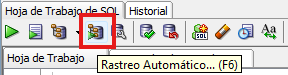
\includegraphics[width=0.5\textwidth]{img/rastreo.png}
\end{center}
\textbf{Ejemplo ventana de rastreo:}
\begin{center}
    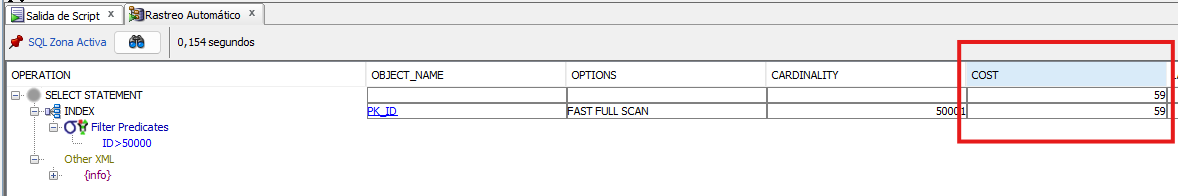
\includegraphics[width=\textwidth]{img/rastreoresultado.png}
\end{center}
\subsubsection{Ver los \'indices de una tabla}
\begin{tcolorbox}[
    colframe=Morado!100, % Color del borde
    colback=Morado!20,       % Color del fondo
    coltitle=white!100, % Color del título
    title=\textbf{PL/SQL}, % Título de la caja
]
    \begin{Verbatim}[breaklines=true]
SELECT * FROM ALL_INDEXES WHERE TABLE_NAME='nombre_tabla';
    \end{Verbatim}
\end{tcolorbox}

\subsubsection{Borrar un \'indice}
\begin{tcolorbox}[
    colframe=red!90!black, % Color del borde
    colback=red!20,       % Color del fondo
    coltitle=white!100, % Color del título
    title=\textbf{PL/SQL}, % Título de la caja
]
    \begin{Verbatim}[breaklines=true]
DROP INDEX <nombre_indice>;
    \end{Verbatim}
\end{tcolorbox}
\end{document}